\documentclass[UTF8,a4paper,12pt]{ctexart}

\usepackage{geometry}
\usepackage{booktabs}
\usepackage{array}
\usepackage{longtable}
\usepackage{graphicx}
\usepackage{float}
\usepackage{hyperref}
\usepackage{xcolor}
\usepackage{listings}
\usepackage{tikz}
\usepackage{amsmath}
\usepackage{enumitem}
\usetikzlibrary{positioning,calc,arrows.meta,fit,backgrounds}

\geometry{left=2.35cm,right=2.35cm,top=2.55cm,bottom=2.55cm}
\hypersetup{colorlinks=true,linkcolor=black,urlcolor=blue}
\setlength{\emergencystretch}{3em}
\setlist{itemsep=0.25em,topsep=0.35em}

\definecolor{ReportBlue}{HTML}{2F5597}
\definecolor{ReportOrange}{HTML}{C55A11}
\definecolor{ReportGreen}{HTML}{548235}
\definecolor{ReportPurple}{HTML}{6F4E7C}
\definecolor{ReportGray}{HTML}{6B7280}
\definecolor{ReportLightGray}{HTML}{E5E7EB}
\definecolor{ReportDark}{HTML}{1F2937}

\lstset{
  basicstyle=\ttfamily\small,
  breaklines=true,
  frame=single,
  columns=fullflexible,
  keepspaces=true,
  showstringspaces=false,
  keywordstyle=\color{ReportBlue},
  commentstyle=\color{ReportGray},
  stringstyle=\color{ReportGreen}
}

\newcommand{\code}[1]{\texttt{#1}}
\newcommand{\seconds}[1]{#1\,s}

\title{并行程序设计 Lab4：MPI 口令猜测并行化与流水线}
\author{姓名：刘蔚霖 \quad 学号：2412727}
\date{\today}

\begin{document}
\maketitle

\begin{abstract}
系统使用消息传递接口（Message Passing Interface，MPI）并行执行概率上下文无关文法
（Probabilistic Context-Free Grammar，PCFG）口令猜测。
Base 版本采用阻塞式 Master-Worker 结构：Rank 0 作为 Master 维护唯一的概率优先队列，将完整预终结式
（Pre-Terminal，PT）动态分配给作为 Worker 的其他 Rank；Worker 生成指定 PT 的候选口令，并使用
ARM NEON 四路单指令多数据流（Single Instruction Multiple Data，SIMD）计算消息摘要算法 5
（Message Digest Algorithm 5，MD5）。
Advanced 版本采用 MPI、POSIX 线程（POSIX Threads，Pthread）与 SIMD 混合并行结构：
Rank 0 的多个生成线程将 PT 切分为
\code{WorkUnit}，经独立有界缓存组成口令批次；Rank 0 主线程使用非阻塞 MPI 请求轮询发送；
加密 Worker 接收批次并执行 NEON MD5。

服务器实验包含单进程基线、阻塞式 MPI 扩展性、流水线 MPI 扩展性、生成线程数、批次大小和问题规模。
所有正式 MPI 任务均正常退出，且每次处理候选口令数均为 10106852。
Base 版本的并行阶段墙钟时间由 1 进程的 \seconds{1.477740} 降至 32 进程的
\seconds{0.236308}，加速比为 6.253。
Advanced 版本在 3 个生成线程时取得该线程实验中的最低墙钟时间 \seconds{1.173190}；
批次上限为 10000 条口令时取得该批次实验中的最低墙钟时间 \seconds{1.096490}。
实验同时表明，Advanced 版本发送完整口令字符串，通信时间占并行阶段墙钟时间的
70.2\%--90.2\%，因此流水线版本慢于发送紧凑 PT 任务的 Base 版本。
\end{abstract}

\tableofcontents
\newpage

\section{并行化目标与实现范围}

\subsection{并行化目标}

PCFG 训练模型记录 PT、字母段、数字段和符号段的概率顺序。
猜测阶段持续从概率优先队列取出 PT，生成候选口令，并计算消息摘要算法 MD5
哈希。

系统使用多个 PT 并行生成口令，并将候选生成、MPI 通信调度和 MD5 加密组织为流水线。
生成进程包含多个具有独立缓存的 Pthread 生成线程，主线程轮询缓存并向多个加密进程发送任务。
加密进程使用 ARM NEON SIMD 计算 MD5。
实验测试不同问题规模、MPI 进程数、生成线程数和批次大小，并分析任务分配、通信开销及并行性能。

表 \ref{tab:requirement-map} 将并行化目标与系统实现和实验依据对应起来。

\begin{longtable}{p{0.22\textwidth}p{0.48\textwidth}p{0.22\textwidth}}
  \caption{MPI 并行化目标与系统实现对应关系}
  \label{tab:requirement-map}\\
  \toprule
  并行化目标 & 系统实现 & 实验依据 \\
  \midrule
  \endfirsthead
  \toprule
  并行化目标 & 系统实现 & 实验依据 \\
  \midrule
  \endhead
  MPI 进程编程 &
  两个 MPI 版本均调用 \code{MPI\_Init\_thread}、\code{MPI\_Comm\_rank}、
  \code{MPI\_Comm\_size} 和 \code{MPI\_Finalize}。 &
  Base 与 Advanced 全部正式任务退出状态为 0。 \\
  多 PT 并行生成 &
  Rank 0 连续调用 \code{PopNextTask()} 扩展优先队列，并同时向多个 Worker 或生成线程分配 PT。 &
  Base 的 NP=1--32 扩展性实验。 \\
  Worker 完成指定 PT 的生成与 MD5 &
  Base Worker 接收序列化 \code{WorkUnit}，调用 \code{GenerateRange()}，随后执行 NEON MD5。 &
  Base 的 Master-Worker 消息协议与处理数量。 \\
  生成与加密流水线 &
  Advanced 的生成线程、Rank 0 MPI 主线程和加密 Worker 同时工作。 &
  Advanced scale 实验。 \\
  生成线程独立缓存结构 &
  Rank 0 默认启动 3 个生成线程，每个线程具有独立任务队列和容量为 2 的 READY 缓存。 &
  \code{GeneratorContext} 与线程数实验。 \\
  MPI 与多线程、SIMD 结合 &
  Rank 0 使用 Pthread 生成；加密 Worker 使用四路 ARM NEON MD5；MPI 负责进程通信。 &
  Advanced 混合并行实现；Backup 对照用于分离加密阶段局部收益。 \\
  探索不同 MPI 编程方法 &
  Base 使用阻塞式 \code{MPI\_Send/MPI\_Recv}；Advanced 使用
  \code{MPI\_Isend/Irecv/Testany/Waitany}。 &
  Base 与 Advanced 性能和通信占比对比。 \\
  负载均衡 &
  Base 将下一完整 PT 交给最先返回的 Worker；Advanced 按预计口令数将切分任务分配给当前累计负载最小的生成线程。 &
  动态调度流程与任务分配函数。 \\
  不同规模、进程数和线程数 &
  支持 \code{--generate}、\code{--gen-threads}、\code{--batch-guesses} 和
  \code{--batch-units}。 &
  问题规模、进程扩展、线程数和批次实验。 \\
  串行与并行性能分析 &
  输出训练、生成关键路径、哈希关键路径、通信和 MPI 墙钟时间。 &
  全部正式实验数据。 \\
  \bottomrule
\end{longtable}

\subsection{代码组织}

系统包含三个可执行版本和一组集中提交脚本：

\begin{itemize}
  \item \code{guess\_mpi\_backup}：单进程基线，用于对比mpi版本实验结果，支持普通 MD5 与四路 NEON SIMD MD5；
  \item \code{guess\_mpi\_base}：阻塞式 Master-Worker MPI 版本；
  \item \code{guess\_mpi\_advanced}：MPI、Pthread 和 SIMD 流水线版本；
  \item \code{submit\_mpi\_batch.sh}：按实验矩阵提交 PBS 作业，并将输出写入各版本的
  \code{data} 目录。
\end{itemize}

两个 MPI 版本共享 \code{WorkUnit}、运行参数解析、MPI 序列化和 MD5 计算接口。
\code{WorkUnit} 包含一个 PT，以及最后一个 segment 的半开区间 $[\mathrm{begin},\mathrm{end})$：

\begin{lstlisting}[language=C++]
struct WorkUnit
{
    PT pt;
    uint64_t begin = 0;
    uint64_t end = 0;
};
\end{lstlisting}

该数据结构同时支持完整 PT 和切分任务。Base 将 \code{begin} 设置为 0，
\code{end} 设置为该 PT 的全部候选数；Advanced 使用 \code{SplitTask()} 按批次上限划分范围。

\section{系统设计}

\subsection{PCFG 模型与任务生成}

训练阶段从 \code{/guessdata/Rockyou-singleLined-full.txt} 读取口令，统计 PT 和 segment value 的频数，
再按概率排序。所有 MPI Rank 独立训练相同模型，Rank 0 输出训练日志。
训练结束后，Rank 0 初始化唯一的 PT 优先队列；各 Rank 通过 \code{MPI\_Barrier} 同步后进入并行阶段。

\code{PopNextTask()} 从队首取出概率最高的 PT，根据 \code{NewPTs()} 产生后继 PT，
计算后继概率并插回队列，随后返回当前 PT。Rank 0 独占这一优先队列，因此 PT 的扩展顺序由单一位置维护。
\code{GuessCount()} 使用 PT 最后一个 segment 的候选 value 数计算任务规模。
\code{GenerateRange()} 固定前序 segment 的当前 value，并枚举最后一个 segment 在指定区间中的 value。
范围生成的关键循环如下。不同 \code{WorkUnit} 使用互不重叠的半开区间，因此可以由不同 Worker
或生成线程独立处理。

\begin{lstlisting}[language=C++]
const uint64_t count = GuessCount(pt);
const uint64_t begin = min(unit.begin, count);
const uint64_t end = min(unit.end, count);

for (uint64_t i = begin; i < end; i += 1)
{
    if (pt.content.size() == 1)
        output.emplace_back(last->ordered_values[i]);
    else
        output.emplace_back(prefix + last->ordered_values[i]);
}
\end{lstlisting}

生成目标采用完整 PT 越过阈值后停止的语义。当目标为 10000000 时，正式实验实际处理
10106852 条候选口令；当目标为 1000000 时，补充实验实际处理 1017695 条候选口令。
\code{Processed guesses} 以实际处理数量为准。

\subsection{公共通信协议与序列化}

MPI 消息通过四个固定 Tag 区分职责，如表 \ref{tab:message-tags} 所示。

\begin{table}[H]
  \centering
  \caption{MPI 消息 Tag}
  \label{tab:message-tags}
  \begin{tabular}{cll}
    \toprule
    Tag & 名称 & 载荷与作用 \\
    \midrule
    100 & \code{TAG\_WORK} & 序列化 \code{WorkUnit}，分配生成与哈希任务 \\
    101 & \code{TAG\_RESULT} & \code{WorkerStats}，返回数量与计时 \\
    102 & \code{TAG\_STOP} & 零字节停止消息 \\
    103 & \code{TAG\_BATCH} & 序列化候选口令批次 \\
    \bottomrule
  \end{tabular}
\end{table}

\code{PT} 和 \code{std::string} 含有动态内存，通信协议使用字段级序列化传输其逻辑内容。
\code{PackWorkUnit()} 使用 \code{MPI\_Pack} 依次写入 segment 数量、segment 类型与长度、
\code{pivot}、当前下标、最大下标、概率和范围边界；接收端按相同顺序调用
\code{MPI\_Unpack} 重建对象。
\code{PackGuessBatch()} 写入口令数量、每条口令长度和字符内容。
该协议使 Base 传输紧凑 PT 描述，使 Advanced 传输已经生成的口令字符串。
下列代码展示 Base 发送 \code{WorkUnit} 的边界。发送前先完成结构化序列化，接收端根据消息长度分配缓冲区，
再重建任务对象。

\begin{lstlisting}[language=C++]
void SendWorkUnitBlocking(int destination, const WorkUnit &unit,
                          MPI_Comm comm)
{
    vector<char> buffer = PackWorkUnit(unit, comm);
    MPI_Send(buffer.data(), buffer.size(), MPI_PACKED,
             destination, TAG_WORK, comm);
}

MPI_Probe(source, MPI_ANY_TAG, comm, &status);
MPI_Get_count(&status, MPI_PACKED, &count);
vector<char> buffer(count);
MPI_Recv(buffer.data(), count, MPI_PACKED, source,
         TAG_WORK, comm, MPI_STATUS_IGNORE);
unit = UnpackWorkUnit(buffer, comm);
\end{lstlisting}

\subsection{MD5 与 SIMD}

MD5 计算默认使用 ARM NEON 四路 SIMD 实现。程序每次将连续四条候选口令交给
\code{MD5Hash\_simdversion()}；不足四条的尾部由普通 \code{MD5Hash()} 处理。
\code{--serial} 参数将全部候选口令切换为普通 MD5。
两个 MPI 版本启动时由 Rank 0 执行普通 MD5 与 SIMD MD5 的正确性测试，再通过
\code{MPI\_Bcast} 将结果广播至所有 Rank。

\section{Base 版本：阻塞式 Master-Worker}

\subsection{进程职责与动态调度}

Base 使用 Rank 0 作为 Master，Rank 1 至 Rank $p-1$ 作为 Worker。
图 \ref{fig:base-flow} 展示了阻塞式消息流程。Master 首先为每个 Worker 分配一个完整 PT；
随后阻塞接收任意 Worker 返回的统计结果，并立即向该 Worker 分配下一个 PT。
当任务耗尽时，Master 向对应 Worker 发送停止消息。

\begin{figure}[H]
  \centering
  \begin{tikzpicture}[
    node distance=0.7cm and 1.4cm,
    box/.style={draw=ReportLightGray, fill=ReportLightGray!25, rounded corners=2pt,
      minimum width=3.0cm, minimum height=0.75cm, align=center, font=\small},
    master/.style={box, draw=ReportBlue, fill=ReportBlue!8},
    worker/.style={box, draw=ReportGreen, fill=ReportGreen!8},
    arrow/.style={-Latex, line width=0.7pt, draw=ReportGray}
  ]
    \node[master] (queue) {Rank 0：PT 优先队列};
    \node[master, below=of queue] (send) {阻塞发送完整 WorkUnit};
    \node[worker, below left=of send] (w1) {Worker 1\\GenerateRange + MD5};
    \node[worker, below=of send] (w2) {Worker 2\\GenerateRange + MD5};
    \node[worker, below right=of send] (wn) {Worker N\\GenerateRange + MD5};
    \node[master, below=2.2cm of send] (recv) {接收任意 Worker 的 WorkerStats\\并立即分配下一 PT};
    \draw[arrow] (queue) -- (send);
    \draw[arrow] (send) -- (w1);
    \draw[arrow] (send) -- (w2);
    \draw[arrow] (send) -- (wn);
    \draw[arrow] (w1) -- (recv);
    \draw[arrow] (w2) -- (recv);
    \draw[arrow] (wn) -- (recv);
    \draw[arrow] (recv.west) -| ([xshift=-1.2cm]send.west) |- (send.west);
  \end{tikzpicture}
  \caption{Base 阻塞式 Master-Worker 消息流程}
  \label{fig:base-flow}
\end{figure}

图 \ref{fig:base-flow} 中，Worker 完成后再领取任务，因而执行较短 PT 的 Worker 不需要等待执行较长 PT 的 Worker。
每个 Worker 以 65536 条候选口令为内部块执行生成和哈希，从而限制临时候选数组的内存占用。
Master 只传输 PT 描述和统计结果，候选口令字符串保留在 Worker 本地。
Worker 的主体循环完成指定 PT 的口令生成和 MD5：

\begin{lstlisting}[language=C++]
static void RunWorker(PriorityQueue &queue,
                      const RuntimeOptions &options)
{
    WorkUnit unit;
    while (ReceiveWorkUnitBlocking(0, unit, MPI_COMM_WORLD))
    {
        const WorkerStats stats =
            ProcessWorkUnit(queue, unit, options.use_simd);
        SendStatsBlocking(0, stats, MPI_COMM_WORLD);
    }
}
\end{lstlisting}

Master 使用 \code{MPI\_ANY\_SOURCE} 接收最先完成的 Worker，并将下一完整 PT 发给该 Worker。
这一循环同时实现多 PT 并行生成和动态负载均衡：

\begin{lstlisting}[language=C++]
const WorkerStats stats =
    ReceiveStatsBlocking(MPI_ANY_SOURCE, &status, MPI_COMM_WORLD);
const int worker = status.MPI_SOURCE;
completed += stats.count;

WorkUnit unit;
if (NextWholePt(queue, options.generate_limit, scheduled, unit))
    SendWorkUnitBlocking(worker, unit, MPI_COMM_WORLD);
else
    SendStopBlocking(worker, MPI_COMM_WORLD);
\end{lstlisting}

\subsection{单进程路径与计时口径}

当 MPI 进程数为 1 时，Rank 0 调用 \code{RunSingleProcess()}，依次生成并哈希完整 PT。
该路径与多进程版本使用相同的 \code{PopNextTask()}、\code{GenerateRange()} 和
\code{HashGuesses()}，因此用于计算 Base 的并行阶段加速比。

Base 输出的 \code{Guess time} 和 \code{Hash time} 分别取所有 Worker 累计生成时间和哈希时间的最大值，
表示两类工作的关键路径。\code{MPI communication/wait time} 统计 Master 阻塞发送、阻塞接收和等待的累计时间。
\code{MPI wall time} 从同步屏障后开始计时，覆盖任务分配、生成、哈希、通信和停止过程。

\section{Advanced 版本：MPI、Pthread 与 SIMD 流水线}

\subsection{三级流水线结构}

Advanced 将并行阶段分成生成、通信调度和加密三个层次。图 \ref{fig:advanced-flow} 展示该流水线结构：
Rank 0 的多个 Pthread 生成候选口令，Rank 0 主线程轮询 READY 缓存并执行 MPI 通信，
加密 Worker 对接收批次执行 NEON MD5。

\begin{figure}[H]
  \centering
  \begin{tikzpicture}[
    node distance=0.65cm and 0.9cm,
    box/.style={draw=ReportLightGray, fill=ReportLightGray!20, rounded corners=2pt,
      minimum width=2.45cm, minimum height=0.72cm, align=center, font=\small},
    gen/.style={box, draw=ReportPurple, fill=ReportPurple!8},
    mpi/.style={box, draw=ReportBlue, fill=ReportBlue!8},
    hash/.style={box, draw=ReportGreen, fill=ReportGreen!8},
    arrow/.style={-Latex, line width=0.7pt, draw=ReportGray}
  ]
    \node[gen] (t0) {生成线程 0\\tasks + READY};
    \node[gen, below=of t0] (t1) {生成线程 1\\tasks + READY};
    \node[gen, below=of t1] (tn) {生成线程 N\\tasks + READY};
    \node[mpi, right=1.5cm of t1] (main) {Rank 0 主线程\\轮询、Pack、Isend/Irecv};
    \node[hash, right=1.5cm of t0] (w1) {加密 Worker 1\\NEON MD5};
    \node[hash, right=1.5cm of main] (w2) {加密 Worker 2\\NEON MD5};
    \node[hash, right=1.5cm of tn] (wn) {加密 Worker N\\NEON MD5};
    \draw[arrow] (t0) -- (main);
    \draw[arrow] (t1) -- (main);
    \draw[arrow] (tn) -- (main);
    \draw[arrow] (main) -- (w1);
    \draw[arrow] (main) -- (w2);
    \draw[arrow] (main) -- (wn);
    \draw[arrow] (w1.west) -| ([xshift=-0.4cm]main.east);
    \draw[arrow] (w2) -- (main);
    \draw[arrow] (wn.west) -| ([xshift=-0.4cm]main.east);
  \end{tikzpicture}
  \caption{Advanced 生成、通信和加密三级流水线}
  \label{fig:advanced-flow}
\end{figure}

每个 \code{GeneratorContext} 保存独立的 \code{tasks} 队列、\code{ready} 队列、
互斥锁和条件变量。READY 队列容量 \code{max\_ready} 为 2。
缓存满时，生成线程通过条件变量等待；Rank 0 主线程取走批次后发出信号。
该有界生产者-消费者结构限制了候选口令批次占用的内存。
以下结构体与等待循环实现生成线程的独立缓存结构：

\begin{lstlisting}[language=C++]
struct GeneratorContext
{
    PriorityQueue *queue = nullptr;
    deque<WorkUnit> tasks;
    deque<GeneratedBatch> ready;
    pthread_mutex_t mutex;
    pthread_cond_t ready_space;
    size_t max_ready = 2;
    uint64_t batch_guesses = 100000;
    int batch_units = 64;
    bool done = false;
};

pthread_mutex_lock(&context.mutex);
while (context.ready.size() >= context.max_ready)
    pthread_cond_wait(&context.ready_space, &context.mutex);
context.ready.emplace_back(std::move(batch));
pthread_mutex_unlock(&context.mutex);
\end{lstlisting}

\subsection{WorkUnit 切分与生成线程负载均衡}

\code{AssignWorkUnits()} 持续从 Rank 0 优先队列获取 PT，并调用
\code{SplitTask(pt, batch\_guesses)} 将大型 PT 切分为多个范围。
程序维护每个生成线程的预计累计口令数，将下一 \code{WorkUnit} 放入当前累计值最小的线程任务队列。
生成线程在候选口令数达到 \code{batch\_guesses}，或合并的任务数达到
\code{batch\_units} 时，将当前批次放入 READY 缓存。

该策略使单个大型 PT 可以分布到多个生成线程。生成线程只调用只读模型上的
\code{GenerateRange()}，每个线程写入自己的局部候选数组和 READY 缓存。
范围切分和最小累计负载分配的关键代码如下：

\begin{lstlisting}[language=C++]
const PT pt = queue.PopNextTask();
const vector<WorkUnit> units =
    queue.SplitTask(pt, options.batch_guesses);

for (const WorkUnit &unit : units)
{
    const size_t index = min_element(assigned.begin(), assigned.end())
                         - assigned.begin();
    contexts[index]->tasks.emplace_back(unit);
    assigned[index] += queue.GuessCount(unit);
}
\end{lstlisting}

\subsection{非阻塞通信与线程级别}

Advanced 通过 \code{MPI\_Init\_thread} 请求
\code{MPI\_THREAD\_FUNNELED} 线程级别。
该线程级别表示多线程进程中只有初始化 MPI 的主线程调用 MPI 接口。
生成线程只执行候选生成和缓存操作；Rank 0 主线程执行全部 MPI 调用。

Rank 0 为每个 Worker 保存独立的发送缓冲区、发送请求、结果接收请求和统计槽位。
主线程取出 READY 批次后，先发布 \code{MPI\_Irecv} 等待结果，再调用
\code{MPI\_Isend} 发送序列化口令批次。\code{MPI\_Testany} 用于轮询完成请求；
全部 Worker 忙碌或生成端排空时，\code{MPI\_Waitany} 等待任意结果。
重新使用某个 Worker 的发送缓冲区前，\code{CompleteWorker()} 调用
\code{MPI\_Wait} 确认对应发送已经完成。
主线程发布非阻塞接收与发送请求的关键代码如下。每个 Worker 使用独立
\code{outbound[worker]} 缓冲区，使缓冲区在发送请求完成前保持有效。

\begin{lstlisting}[language=C++]
outbound[worker] = PackGuessBatch(batch.guesses, MPI_COMM_WORLD);
MPI_Irecv(&result_slots[worker], sizeof(WorkerStats), MPI_BYTE,
          worker, TAG_RESULT, MPI_COMM_WORLD,
          &result_requests[worker]);
MPI_Isend(outbound[worker].data(), outbound[worker].size(), MPI_PACKED,
          worker, TAG_BATCH, MPI_COMM_WORLD,
          &send_requests[worker]);

MPI_Testany(world_size, result_requests.data(), &completed_worker,
            &completed_flag, MPI_STATUS_IGNORE);
\end{lstlisting}

\section{实验环境与方法}

\subsection{运行环境与编译}

实验通过作业系统提交至 ARM 计算节点。每个计算节点最多申请 8 个核心，
实验申请节点数不超过 4。MPI 程序使用 MPICH 提供的
\code{/usr/local/bin/mpiexec} 启动，PBS 的 \code{PBS\_NODEFILE} 描述分配的节点和槽位。
Advanced 作业脚本按轮询顺序生成临时 machinefile，使 MPI Rank 在多节点配置中均匀分布。

三个版本使用 \code{-O2} 编译：

\begin{lstlisting}[language=bash]
# Backup
g++ -O2 main.cpp train.cpp guessing.cpp md5.cpp -o main -fopenmp

# Base
mpic++ -O2 main.cpp train.cpp guessing.cpp md5.cpp mpi_support.cpp \
  -o main -fopenmp

# Advanced
mpic++ -O2 main.cpp train.cpp guessing.cpp md5.cpp mpi_support.cpp \
  -o main -pthread -fopenmp
\end{lstlisting}

\subsection{实验矩阵（批量提交实验任务）}

表 \ref{tab:experiment-matrix} 给出正式实验矩阵。除 Backup 外，每个正式 MPI 配置运行 3 次并取中位数；
Backup 的普通 MD5 与 SIMD MD5 各运行 5 次并取中位数。

\begin{table}[H]
  \centering
  \caption{实验矩阵}
  \label{tab:experiment-matrix}
  \small
  \begin{tabular}{p{0.24\textwidth}p{0.35\textwidth}p{0.24\textwidth}}
    \toprule
    实验组 & 配置 & 目的 \\
    \midrule
    Backup Hash & Serial、NEON SIMD，各 5 次 & 分离 SIMD 的 MD5 局部收益 \\
    Base Scale & NP=1/2/4/8/16/32，各 3 次 & 阻塞式 MPI 扩展性 \\
    Advanced Scale & NP=2/4/8/16，3 生成线程，各 3 次 & 流水线 MPI 扩展性 \\
    Advanced Threads & NP=4，生成线程=1/2/3/4，各 3 次 & MPI 流水线生成端线程数敏感性 \\
    Advanced Batch & NP=4，批次=10k/50k/100k/500k，各 3 次 & 任务粒度与通信分析 \\
    Advanced Size & NP=4，目标 1M，单次补充实验 & 问题规模检查 \\
    \bottomrule
  \end{tabular}
\end{table}

Base 与 Advanced 的正式 10M 实验每次均处理 10106852 条候选口令。
Advanced Size 实验处理 1017695 条候选口令。
所有正式任务和补充任务均输出 \code{Exit status: 0}；错误输出中只有服务器授权提示。

\subsection{指标定义}

训练阶段结束后的 MPI 并行阶段是本实验的主要评价范围。原因是每个 Rank 独立训练完整模型，
每个 Rank 独立执行训练过程，共享服务器上的训练时间受节点负载影响明显。
实验使用以下指标：

\begin{align}
S(p) &= \frac{T_{\mathrm{Base},1}}{T_{\mathrm{Base},p}},\\
E(p) &= \frac{S(p)}{p},\\
R_{\mathrm{comm}} &= \frac{T_{\mathrm{comm}}}{T_{\mathrm{wall}}},\\
Q &= \frac{N_{\mathrm{processed}}}{T_{\mathrm{wall}}}.
\end{align}

其中 $T_{\mathrm{wall}}$ 为 \code{MPI wall time}，$S(p)$ 为 Base 相对单进程路径的加速比，
$E(p)$ 为并行效率，$R_{\mathrm{comm}}$ 为通信时间占比，$Q$ 为有效吞吐率。
\code{Guess time} 和 \code{Hash time} 表示对应工作在生成线程或 Worker 上的关键路径，
两者与通信阶段存在时间重叠，MPI 墙钟时间记录整个并行阶段的实际持续时间。

并行加速取决于计算时间节省量与附加开销之间的关系。将 Master 串行工作、MPI 通信、
负载不均衡造成的尾部等待和其他固定开销合并为 $T_{\mathrm{overhead}}(p)$，则进程数为 $p$
时的并行阶段可表示为
\[
T_p = T_{\mathrm{parallel}}(p) + T_{\mathrm{overhead}}(p).
\]
当并行计算缩短的时间大于 $T_{\mathrm{overhead}}(p)$ 时，墙钟时间下降并形成加速；
当新增进程主要增加调度、通信或等待时，墙钟时间保持不变或上升。后续分析使用墙钟时间判断整体加速，
并结合生成、哈希和通信计时定位性能边界。

Backup 的停止检查位于最终批次哈希之前，其 Hash 时间不覆盖最后一批候选口令。
Backup Serial 与 Backup SIMD 使用相同计时边界，用于比较 MD5 实现的局部性能。
MPI 加速比以 Base 的单进程路径为基准。

\section{正确性与完整性验证}

程序启动时执行普通 MD5 与 SIMD MD5 正确性测试；正式实验还检查处理数量、退出状态和错误输出。
表 \ref{tab:correctness} 汇总验证结果。

\begin{table}[H]
  \centering
  \caption{正确性与任务完整性}
  \label{tab:correctness}
  \begin{tabular}{lccc}
    \toprule
    实验组 & 成功任务数 & 正式处理数量 & 退出状态 \\
    \midrule
    Backup Serial/SIMD & 10/10 & 10106852 & 正常 \\
    Base Scale & 18/18 & 10106852 & 正常 \\
    Advanced Scale & 12/12 & 10106852 & 正常 \\
    Advanced Threads & 12/12 & 10106852 & 正常 \\
    Advanced Batch & 12/12 & 10106852 & 正常 \\
    Advanced Size & 1/1 & 1017695 & 正常 \\
    \bottomrule
  \end{tabular}
\end{table}

Base 和 Advanced 在不同进程数、线程数和批次参数下均得到相同的正式处理数量。
一致的处理数量表明 PT 动态调度、范围切分、批次传输和非阻塞请求保持了任务统计完整性。

\section{性能结果与分析}

\subsection{加密 Worker 局部性能与流水线瓶颈}

图 \ref{fig:simd-hash} 展示单进程 Backup 中普通 MD5 与 NEON SIMD MD5 的 Hash 时间中位数。
两种模式处理相同生成流程，并使用相同计时边界。

\begin{figure}[H]
  \centering
  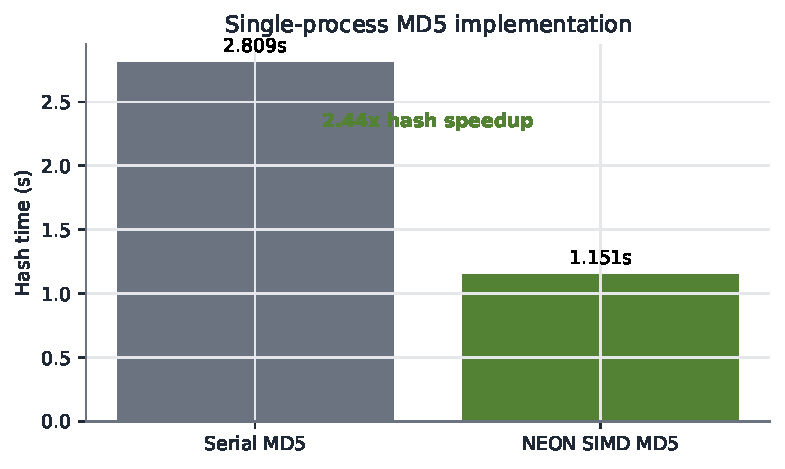
\includegraphics[width=0.64\textwidth]{assets/simd_hash.pdf}
  \caption{普通 MD5 与 ARM NEON SIMD MD5 的 Hash 时间}
  \label{fig:simd-hash}
\end{figure}

普通 MD5 的 Hash 时间中位数为 \seconds{2.808640}，NEON SIMD MD5 为
\seconds{1.150800}，局部加速比为 2.441。
该结果说明四路 NEON 能降低加密 Worker 的计算时间；当 MPI 通信或候选生成成为主要开销时，
整体性能仍由流水线中的较慢阶段决定。该对照反映 MPI 混合并行结构中加密阶段的计算能力。
SIMD 加速作用于 MD5 计算部分，PT 扩展、候选生成、任务调度和 MPI 通信仍按各自路径执行。
因此，2.441 倍是加密阶段的局部加速比，整体墙钟时间的加速上限同时受其余阶段占比约束。

\subsection{Base 进程扩展性}

表 \ref{tab:base-scale} 给出 Base 的中位数结果。NP=1 使用相同生成与哈希接口执行单进程路径，
其 MPI 墙钟时间作为加速比基准。

\begin{table}[H]
  \centering
  \caption{Base 进程扩展性（3 次中位数）}
  \label{tab:base-scale}
  \small
  \begin{tabular}{rrrrrrr}
    \toprule
    NP & Guess(s) & Hash(s) & Comm/Wait(s) & Wall(s) & Speedup & Efficiency \\
    \midrule
    1  & 0.177645 & 1.079900 & 0.000000 & 1.477740 & 1.000 & 100.0\% \\
    2  & 0.198691 & 1.083920 & 1.318610 & 1.553260 & 0.951 & 47.6\% \\
    4  & 0.068480 & 0.363594 & 0.352613 & 0.550390 & 2.685 & 67.1\% \\
    8  & 0.037242 & 0.168138 & 0.098765 & 0.328883 & 4.493 & 56.2\% \\
    16 & 0.026160 & 0.124169 & 0.042525 & 0.263377 & 5.611 & 35.1\% \\
    32 & 0.017396 & 0.093723 & 0.043122 & 0.236308 & 6.253 & 19.5\% \\
    \bottomrule
  \end{tabular}
\end{table}

图 \ref{fig:base-scaling} 同时展示墙钟时间、加速比和效率。误差线使用每组 3 次运行的最小值与最大值。

\begin{figure}[H]
  \centering
  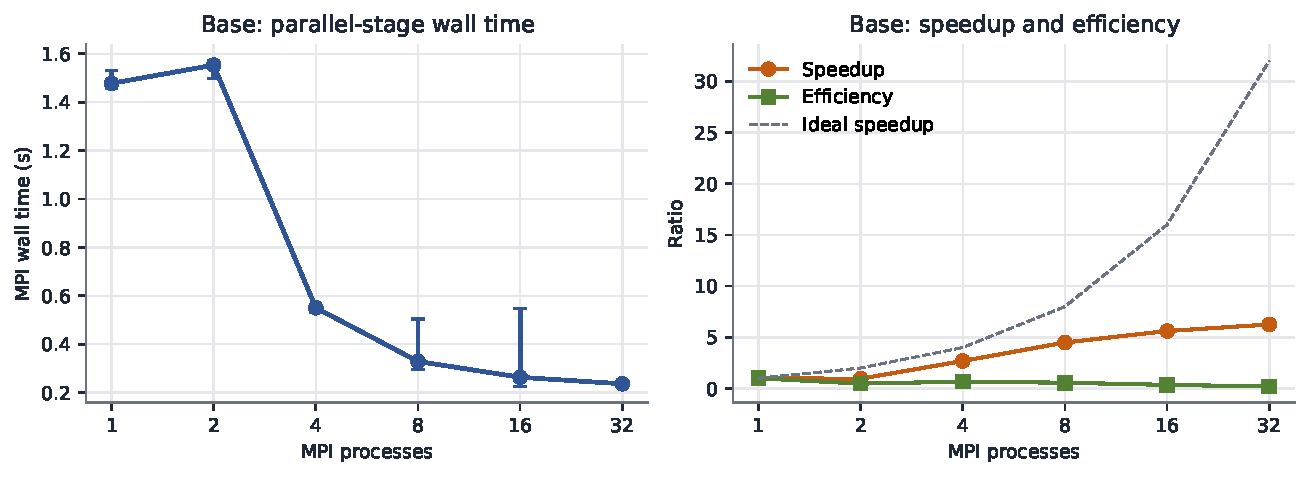
\includegraphics[width=0.98\textwidth]{assets/base_scaling.pdf}
  \caption{Base 的 MPI 并行阶段扩展性}
  \label{fig:base-scaling}
\end{figure}

NP=2 时只有一个 Worker，Rank 0 专门负责调度，因此可用于生成和哈希的计算进程仍为 1；
同时增加了阻塞通信，墙钟时间由 \seconds{1.477740} 增至 \seconds{1.553260}。
该配置的生成和哈希关键路径分别比 NP=1 高 11.8\% 和 0.4\%，
\code{Comm/Wait} 占墙钟时间 84.9\%。一个计算 Worker 没有增加并行计算能力，
Master-Worker 消息和进程切换使 NP=2 的加速比为 0.951，形成减速。

NP=4 时有 3 个 Worker 同时处理不同 PT。生成关键路径比 NP=1 降低 61.5\%，
哈希关键路径降低 66.3\%，墙钟时间降低 62.8\%，对应 2.685 倍加速。
这一配置已经具有多个计算 Worker，且 Master 传输紧凑 PT 描述，Worker 本地生成候选口令，
计算时间节省量超过了调度与通信开销。

NP 从 4 增至 32 时，生成与哈希关键路径持续下降，32 进程墙钟时间为
\seconds{0.236308}，相对 NP=1 加速 6.253 倍。
从 NP=8 增至 NP=32 使用了 4 倍进程资源，墙钟时间由 \seconds{0.328883} 降至
\seconds{0.236308}，仅继续下降 28.2\%。NP=16 至 NP=32 的墙钟时间下降 10.3\%，
并行效率同时从 35.1\% 降至 19.5\%。此阶段生成与哈希关键路径已经较短，
Rank 0 串行扩展与分配 PT、完整 PT 之间的规模差异、末尾少量任务造成的尾部等待以及固定消息开销
占据更高比例，因此继续增加进程仍能加速，但边际收益持续下降。

\code{Comm/Wait} 记录 Master 的阻塞通信与等待时间，其中包含 Worker 正在执行本地生成和哈希时
Master 的等待，因此该指标描述控制路径占用，数值并非纯网络传输时间。
Base 在 NP=32 时该指标为 \seconds{0.043122}，紧凑 PT 描述使消息载荷保持较小；
扩展性上限更多来自中心 Master 和任务粒度，而非完整候选口令的网络传输。

\subsection{Base 与 Advanced 通信方法对比}

图 \ref{fig:version-compare} 比较共同进程数下的 Base 和 Advanced，并给出通信时间占 MPI 墙钟时间的比例。
Base 传输紧凑 \code{WorkUnit}，Worker 在本地生成并哈希；Advanced 在 Rank 0 生成口令后传输完整字符串批次。

\begin{figure}[H]
  \centering
  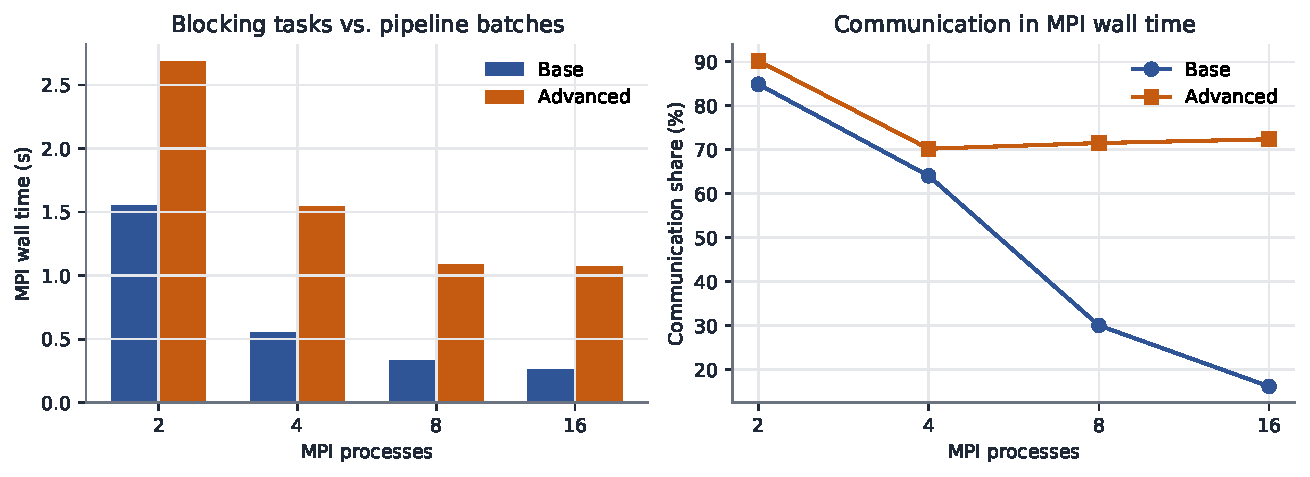
\includegraphics[width=0.98\textwidth]{assets/version_compare.pdf}
  \caption{Base 与 Advanced 的墙钟时间和通信占比}
  \label{fig:version-compare}
\end{figure}

表 \ref{tab:advanced-scale} 给出 Advanced 的进程扩展结果。

\begin{table}[H]
  \centering
  \caption{Advanced 进程扩展性（3 次中位数，3 个生成线程）}
  \label{tab:advanced-scale}
  \small
  \begin{tabular}{rrrrrr}
    \toprule
    NP & Guess(s) & Hash(s) & Communication(s) & Wall(s) & 通信占比 \\
    \midrule
    2  & 0.119535 & 1.122440 & 2.419430 & 2.682270 & 90.2\% \\
    4  & 0.192703 & 0.404577 & 1.083050 & 1.542380 & 70.2\% \\
    8  & 0.144236 & 0.266076 & 0.775140 & 1.083920 & 71.5\% \\
    16 & 0.142998 & 0.247190 & 0.775905 & 1.072140 & 72.4\% \\
    \bottomrule
  \end{tabular}
\end{table}

Advanced 的墙钟时间从 NP=2 的 \seconds{2.682270} 降至 NP=16 的
\seconds{1.072140}，说明多个加密 Worker 可以并行处理批次。
NP=2 至 NP=4 期间，哈希关键路径降低 64.0\%，通信时间降低 55.2\%，墙钟时间降低 42.5\%；
增加的加密 Worker 能够并行消费 Rank 0 生成的口令批次，因此该区间形成明显加速。
NP=4 至 NP=8 期间，哈希关键路径继续降低 34.2\%，墙钟时间降低 29.7\%，
表明加密计算仍是可并行部分。

NP 从 8 增至 16 时墙钟时间仅下降 1.1\%，而通信时间保持在约 \seconds{0.776}；
哈希关键路径仅继续降低 7.1\%。此时增加加密 Worker 缩短的计算时间已经小于
Rank 0 的批次打包、发送、请求完成处理和网络传输开销，因而扩展进入饱和区间。
共同进程数下，Advanced 均慢于 Base。该差异来自两种协议的数据粒度：
Base 发送 PT 描述，Advanced 发送每条候选口令的长度和字符内容。
在 NP=4、8 和 16 时，Advanced 墙钟时间分别为 Base 的 2.80、3.30 和 4.07 倍；
进程数增加后差距扩大，说明完整口令批次的数据移动成本随 Worker 数增加成为更明显的限制。

\subsection{生成线程数}

线程数实验固定 NP=4、\code{batch\_guesses=100000} 和
\code{batch\_units=64}。图 \ref{fig:advanced-tuning} 左侧展示生成线程数对墙钟时间和生成关键路径的影响。

\begin{figure}[H]
  \centering
  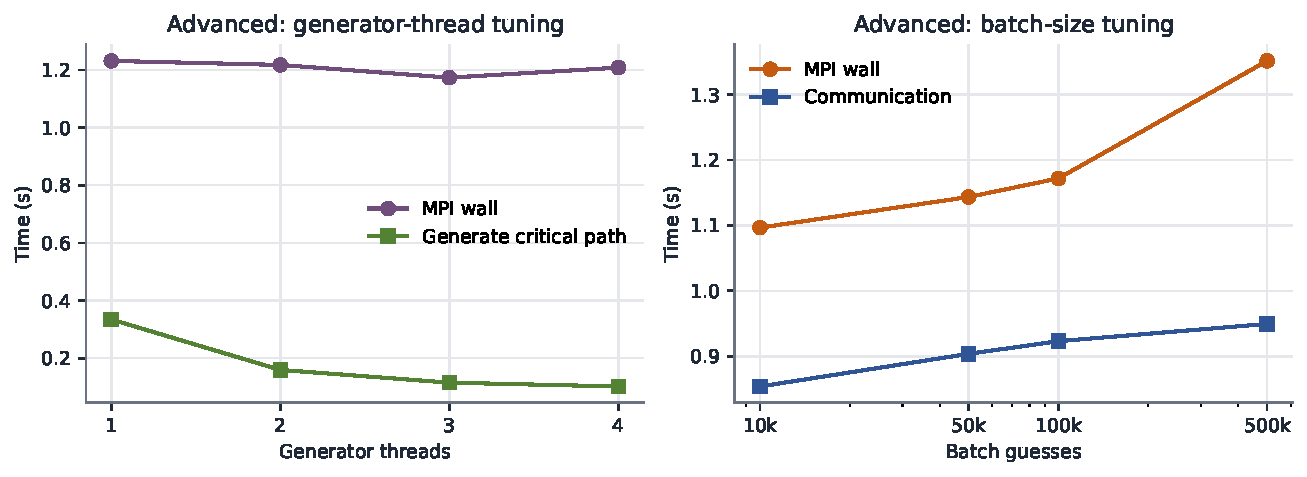
\includegraphics[width=0.98\textwidth]{assets/advanced_tuning.pdf}
  \caption{Advanced 的生成线程数与批次大小参数实验}
  \label{fig:advanced-tuning}
\end{figure}

表 \ref{tab:threads} 给出线程数实验的中位数。生成线程从 1 增至 3 时，
生成关键路径由 \seconds{0.334514} 降至 \seconds{0.115355}，MPI 墙钟时间由
\seconds{1.231360} 降至 \seconds{1.173190}。4 个生成线程将生成关键路径继续降至
\seconds{0.102094}，但墙钟时间回升至 \seconds{1.207960}。

\begin{table}[H]
  \centering
  \caption{Advanced 生成线程数实验（NP=4，3 次中位数）}
  \label{tab:threads}
  \begin{tabular}{rrrrr}
    \toprule
    生成线程 & Guess(s) & Hash(s) & Communication(s) & Wall(s) \\
    \midrule
    1 & 0.334514 & 0.375961 & 0.976711 & 1.231360 \\
    2 & 0.159553 & 0.378193 & 0.973121 & 1.217270 \\
    3 & 0.115355 & 0.370383 & 0.932171 & 1.173190 \\
    4 & 0.102094 & 0.379805 & 0.963883 & 1.207960 \\
    \bottomrule
  \end{tabular}
\end{table}

该结果表明，生成线程能够降低生成关键路径，但 NP=4 配置的墙钟时间主要受通信影响。
生成线程从 1 增至 3 时，生成关键路径降低 65.5\%，墙钟时间仅降低 4.7\%；
生成阶段的显著缩短没有等比例传递到整体时间，说明通信和加密阶段决定了主要等待时间。
从 3 个线程增至 4 个线程时，生成关键路径继续降低 11.5\%，墙钟时间反而上升 3.0\%。
额外线程会与 Rank 0 MPI 主线程争用处理器和内存带宽，同时生成端已经能够持续提供批次，
因此 4 个线程没有形成整体加速。3 个生成线程在本组参数中取得最低墙钟时间。

\subsection{批次大小}

图 \ref{fig:advanced-tuning} 右侧和表 \ref{tab:batch} 展示批次大小实验。
实验固定 NP=4、3 个生成线程和 \code{batch\_units=64}。

\begin{table}[H]
  \centering
  \caption{Advanced 批次大小实验（NP=4，3 次中位数）}
  \label{tab:batch}
  \begin{tabular}{rrrrr}
    \toprule
    Batch guesses & Guess(s) & Hash(s) & Communication(s) & Wall(s) \\
    \midrule
    10000  & 0.066483 & 0.361774 & 0.853921 & 1.096490 \\
    50000  & 0.084996 & 0.371753 & 0.903782 & 1.143310 \\
    100000 & 0.115477 & 0.376951 & 0.923059 & 1.171710 \\
    500000 & 0.564914 & 0.411472 & 0.949456 & 1.351160 \\
    \bottomrule
  \end{tabular}
\end{table}

批次上限为 10000 条口令时墙钟时间最低，为 \seconds{1.096490}。
批次增至 500000 时，生成关键路径增至 \seconds{0.564914}，墙钟时间增至
\seconds{1.351160}，比 10000 条配置高 23.2\%。
生成线程在达到批次数量或任务数阈值后发布 READY 批次；
大批次延长了批次可发送前的等待时间，并增加了尾部批次的不均衡程度。
较大批次能够减少消息次数，但本组实验中消息次数节省量没有抵消批次组装等待和尾部不均衡。
10000 条配置更早向 Worker 发布工作，使生成、传输和加密保持更细粒度的重叠。
该结果表明批次合并只有在消息启动开销占主导时能够形成加速；当前实现的主要成本还包括完整字符串序列化
与传输，因此单纯增大批次无法消除数据移动开销。

\subsection{问题规模}

问题规模实验固定 Advanced NP=4、3 个生成线程、
\code{batch\_guesses=100000} 和 \code{batch\_units=64}。
图 \ref{fig:problem-size} 将目标 1M 的单次补充结果与目标 10M 的正式 scale 中位数并列展示。

\begin{figure}[H]
  \centering
  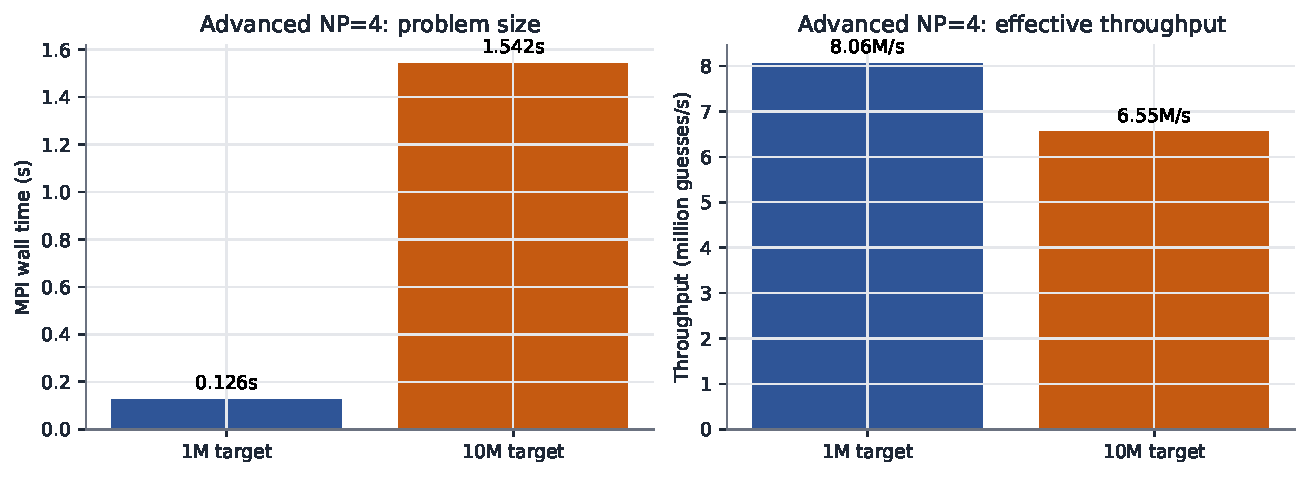
\includegraphics[width=0.98\textwidth]{assets/problem_size.pdf}
  \caption{Advanced NP=4 在两个问题规模下的墙钟时间和吞吐率}
  \label{fig:problem-size}
\end{figure}

目标 1M 实际处理 1017695 条候选口令，MPI 墙钟时间为 \seconds{0.126246}；
目标 10M 实际处理 10106852 条候选口令，MPI 墙钟时间中位数为 \seconds{1.542380}。
两组有效吞吐率分别约为 8.06 和 6.55 百万条/秒。
1M 数据包含一次运行，且两组任务处于共享服务器的不同作业批次，因此该图用于确认不同规模参数的执行行为；
稳定的规模效率分析需要补充同一作业条件下的重复实验。
10M 任务的处理数量约为 1M 任务的 9.93 倍，墙钟时间约为其 12.22 倍。
该次结果没有表现出问题规模增大带来的吞吐率提升；共享服务器波动、批次序列化和较长任务中的持续通信
共同影响观测值。固定启动开销在更大问题规模中占比下降，但完整口令的数据移动量随处理数量同步增长，
因此扩大问题规模本身不会消除 Advanced 的通信瓶颈。

\subsection{训练时间与共享服务器波动}

每个 Rank 独立训练完整 PCFG 模型，训练阶段在 MPI 墙钟计时之前完成。
不同配置的 Rank 数和节点数不同，训练期间会同时读取训练集并占用计算资源；
共享服务器负载也会影响训练时间。Base 的训练时间中位数在
\seconds{26.3415} 至 \seconds{45.3495} 之间，Advanced scale 在
\seconds{27.1115} 至 \seconds{33.2332} 之间。

MPI 墙钟时间用于分析并行阶段，训练时间单独报告。
端到端运行时间可写为
\[
T_{\mathrm{end-to-end}} = T_{\mathrm{train}} + T_{\mathrm{MPI\ wall}},
\]
该指标主要反映独立训练和共享环境状态；MPI 调度方法的评价采用并行阶段墙钟时间和通信时间。
以 Base 各配置的中位数计算，MPI 阶段仅占训练时间与 MPI 墙钟时间之和的约
0.6\%--5.3\%。训练过程由每个 Rank 独立执行，进程数增加不会缩短该阶段，
并且多 Rank 同时读取训练集和计算模型会增加共享资源竞争。
因此，Base 的 6.253 倍加速明确作用于口令生成与 MD5 的 MPI 并行阶段；
端到端运行时间主要由训练阶段决定，无法获得同等幅度的整体加速。

\section{系统特性与性能边界}

\subsection{负载均衡机制}

Base 的动态调度根据 Worker 完成顺序分配完整 PT，适用于 PT 数量较多且单个 PT 大小可接受的场景。
其通信载荷紧凑，提前完成的 Worker 能够持续领取任务。
Advanced 将大型 PT 切分为范围任务，并按预计候选数平衡生成线程负载，从而实现生成与加密重叠；
Rank 0 同时承担生成、打包和发送，因此通信与中心节点处理能力限制整体扩展性。

\subsection{通信方法的适用范围}

阻塞式通信使 Base 的控制流直接：Master 每次等待一个结果后分配下一任务。
Base 在 NP=32 时通信等待时间中位数为 \seconds{0.043122}，占 MPI 墙钟时间 18.2\%。
Advanced 的非阻塞请求使 Rank 0 能同时维护多个发送、接收和 READY 缓存。
Advanced 的通信占比在 70.2\%--90.2\% 之间，说明性能边界主要来自完整口令批次的序列化和传输。



\subsection{综合结果}

Base 的 Rank 0 独占 PT 优先队列并连续扩展多个 PT。Master 使用阻塞式 MPI 消息将完整 PT
动态分配给 Worker，Worker 在本地完成指定 PT 的候选生成与 NEON MD5。该结构在 NP=1--32
配置下保持处理数量一致，并在 NP=32 时取得 6.253 的并行阶段加速比。

Advanced 使用 Pthread 生成线程、独立有界缓存和 SIMD 加密 Worker 构成 MPI 混合并行流水线。
主线程使用非阻塞发送、接收和完成请求连接加密 Worker。大型 PT 通过 \code{WorkUnit} 范围切分，
并按预计候选数平衡生成线程负载。3 个生成线程和 10000 条口令批次分别取得对应参数实验中的最低墙钟时间。
完整口令批次的序列化与传输使通信时间占比达到 70.2\%--90.2\%。

\clearpage
\section{结论}

系统包含两种 MPI 口令猜测并行结构。Base 使用阻塞式 Master-Worker 协议，
Rank 0 维护唯一 PT 优先队列，Worker 完成完整 PT 的候选生成和 NEON MD5。
Base 的 MPI 墙钟时间从 NP=1 的 \seconds{1.477740} 降至 NP=32 的
\seconds{0.236308}，并行阶段加速比为 6.253。NP=2 只有一个计算 Worker，
新增的 Master-Worker 通信使加速比为 0.951；NP=4 开始具有多个计算 Worker，
生成和哈希关键路径分别降低 61.5\% 和 66.3\%，形成 2.685 倍加速。
NP=8 至 NP=32 仍持续缩短墙钟时间，但中心 Master、PT 粒度差异和尾部等待使并行效率降至 19.5\%。

Advanced 使用 MPI、Pthread 和 SIMD 三级流水线，生成线程通过独立有界缓存向 Rank 0 主线程提供批次，
主线程使用非阻塞 MPI 请求连接加密 Worker。NP=2 至 NP=8 期间，增加加密 Worker 能够降低哈希关键路径，
墙钟时间从 \seconds{2.682270} 降至 \seconds{1.083920}。NP=8 至 NP=16 期间，
哈希关键路径仅继续降低 7.1\%，墙钟时间仅下降 1.1\%，流水线进入通信饱和区间。
Advanced 的通信时间占 MPI 墙钟时间的 70.2\%--90.2\%，完整口令批次的序列化与传输构成性能边界。
Base 传输紧凑 PT 描述，并在 Worker 本地完成生成与哈希，因此具有更低的并行阶段墙钟时间。

参数实验显示，增加资源只有在对应阶段限制墙钟时间时才能形成整体加速。
生成线程从 1 增至 3 时生成关键路径降低 65.5\%，墙钟时间降低 4.7\%；继续增加至 4 个线程后，
资源竞争使墙钟时间回升 3.0\%。批次上限为 10000 条口令时取得最低墙钟时间；
批次增至 500000 条后，批次组装等待和尾部不均衡使墙钟时间增加 23.2\%。
NEON SIMD 将 MD5 局部计算加速 2.441 倍，其整体收益受候选生成、MPI 通信和调度开销约束。

训练阶段由每个 Rank 独立执行，其中位数为数十秒，而 MPI 并行阶段仅占训练时间与 MPI 墙钟时间之和的
约 0.6\%--5.3\%。因此，本实验的 MPI 加速主要作用于训练完成后的口令生成和 MD5 搜索阶段；
端到端性能的进一步提升需要并行化训练过程或复用已训练模型。

\end{document}
